\documentclass[xcolor=dvipsnames,slidestop,compress,mathserif,color]{beamer}
\usepackage[english]{babel}
\usepackage[utf8]{inputenc}
\usepackage{listings}
\usepackage[noend]{algorithmic}


\useoutertheme[subsection=false,footline=authortitle]{miniframes}
\useinnertheme[shadow]{rounded}
\usecolortheme{orchid}
\setbeamercolor{separation line}{use=structure,bg=structure.fg!50!bg}


\logo{
\includegraphics[height=1cm]{../images/logo_inf}}

\title[ACS Component Code Generator]{ACS Component Code Generator}
\author[Troncoso]{
\mbox{Nicol\'as Troncoso}}
\institute[UTFSM]{
Departamento de Inform\'atica\\
Universidad T\'ecnica Federico Santa Mar\'ia}
\date[ICI]{\tiny{Thesis Presented in Partial Fulfillment of the Requirements
for the Engineering Degree}\\ \Large{Ingeniero Civil en Inform\'atica}}

\makeindex

\newenvironment<>{varblock}[2][\textwidth]{%
  \setlength{\textwidth}{#1}
  \begin{actionenv}#3%
    \def\insertblocktitle{#2}%
    \par%
    \usebeamertemplate{block begin}}
  {\par%
    \usebeamertemplate{block end}%
  \end{actionenv}}

\begin{document}

\begin{frame}
\titlepage
\end{frame}


\begin{frame}
\frametitle{Contents}
\tableofcontents
%\begin{columns}
%\begin{column}{0.5\textwidth}
%\tableofcontents[sections={1-3}]
%\end{column}
%\begin{column}{0.5\textwidth}
%\tableofcontents[sections={4-8}]
%\end{column}
%\end{columns}
\end{frame}


\section[What is ACS?]{What is ACS?}
\begin{frame}
\frametitle{ACS Definition}
\only<1>{
  \begin{block}{Technical Description}<1>
    \begin{itemize}
      \item Component/Conatiner Framework.
      \item Common Services.
      \item Portability through CORBA.
    \end{itemize}
  \end{block}
}
\only<2>{
  \begin{block}{Human Description}<2>
    \begin{itemize}
      \item An International Restuarant.
      \item Has a Salad Bar.
      \item Service speaks many languages.
    \end{itemize}

  \end{block}
}
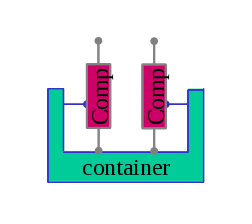
\includegraphics{comp-cont}
\end{frame}

\subsection[Component/Container]{Component/Container Framework}
\begin{frame}
\frametitle{Operations}
  
\only<1>{
  \begin{block}{Lifecycle}
    \begin{itemize}
       \item\texttt{init()}
       \item\texttt{stop()}
       \item\texttt{cleanup()}
    \end{itemize}
  \end{block}
   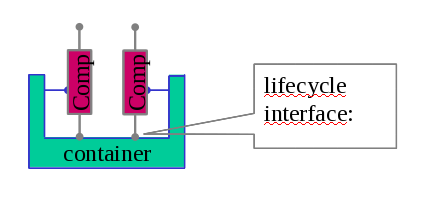
\includegraphics{lifecycle}
    }
\only<2>{
  \begin{block}{Container services}
    \begin{itemize}
       \item\texttt{getComponent(otherComp)}
       \item\texttt{getLogger()}
       \item Access the Notification Channel.
    \end{itemize}
  \end{block}
   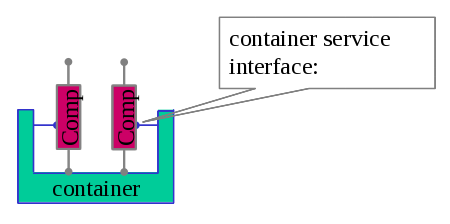
\includegraphics{services}
    }
\end{frame}

\subsection[Usage]{Where is it Used?}
\begin{frame}
\frametitle{Actual Sites}
   \includegraphics<1>[height=6cm]{HPT}
   \includegraphics<2>[height=6cm]{APEX}
   \includegraphics<3>[height=3cm]{ALMA}
\end{frame}



\section[Problem Description]{Problem Description and Scope}
\begin{frame}
\frametitle{Problem Description and Scope}
\begin{block}{Components}<1->
   \begin{itemize}
      \item Power Supply
      \item Telescope Mount
      \item Alarm Clock
      \item Coffee Machine
   \end{itemize}
\end{block}
  \uncover<2->{\textbf{They all interact the same way with ACS}}
\begin{varblock}[0.9\textwidth]{Common Attributes}<3->
   \begin{itemize}
      \item implement LifeCycle
      \item use Container Services
   \end{itemize}
\end{varblock}
\end{frame}

\subsection[Complexity]{Complexity of the Framework}
\begin{frame}
\frametitle{Thing to Have in Mind}
\begin{itemize}
   \item<1->{3+1 programing languages.}
   \uncover<2->{
       \begin{itemize}
          \item \texttt{C++}
          \item \texttt{Java}
          \item \texttt{Python}
          \item \texttt{IDL}
       \end{itemize}
   }
   \item<3->{Definition of the Configuration DatabBase (CDB).}
   \item<4->{Definition of XML Schemas.}
   \item<5->{ACS services and how to use them}
   \item<6->{Learning curve of knowing how it all fits together}
\end{itemize}

\end{frame}
%\subsection[Model Driven]{Model Driven Architecture}
\section[Solution]{Solution of Our Problems}
\begin{frame}
\frametitle{Solution Objective}
\vspace{1.2cm}
\begin{block}{Tools}
Automatically generate as much implementation as possible for an 
ACS component.
\only<2>{
\begin{itemize}
\item UML 2.0 in XMI format.
\item Open Architecture Ware (OAW)
\end{itemize}
}
\end{block}
\end{frame}

\begin{frame}
\frametitle{Solution Requirements}
\begin{block}{Design}<1->
\begin{itemize}
\item Model Driven Generation
\end{itemize}
\end{block}
\only<1>{
\begin{figure}
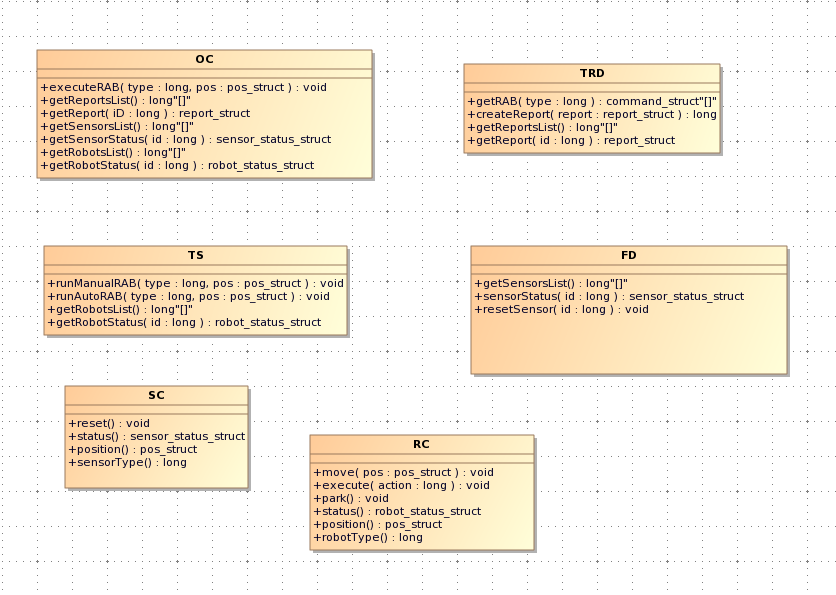
\includegraphics[width=0.7\textwidth]{MARS-classdiagram-full}
\end{figure}
}
\only<2>{
\begin{figure}
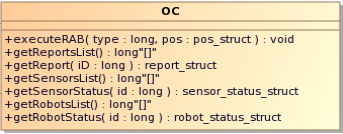
\includegraphics[width=0.7\textwidth]{MARS-zoom}
\end{figure}
}
\only<3>{
\begin{figure}
\includegraphics[height=0.65\textheight]{general-workflow}
\end{figure}
}
\end{frame}
\subsection[Design]{Solution Design}
\begin{frame}
\begin{varblock}[0.9\textwidth]{How is it done?}
\begin{center}
\includegraphics[height=0.68\textwidth]{design}
\end{center}
\end{varblock}
\end{frame}

\begin{frame}[fragile]
\begin{varblock}[0.9\textwidth]{Template}
\begin{verbatim}
«IMPORT uml»
«EXTENSION templates::util»

«DEFINE Root FOR uml::Model»
«FILE 'idl/'+this.name+"Common.idl"»
#ifndef «this.name»_IDL
#define «this.name»_IDL
#pragma prefix "alma"

module «this.name»
{
«FOREACH allOwnedElements().
      typeSelect(uml::Enumeration) AS element»
        «EXPAND ENUM FOR element»
«ENDFOREACH-»
\end{verbatim}
\end{varblock}
\end{frame}
\begin{frame}[fragile]
\begin{varblock}[0.9\textwidth]{Template}
\begin{verbatim}
«DEFINE ENUM FOR uml::Enumeration»
    enum «this.name» {
    «FOREACH  this.eAllContents.
          typeSelect(uml::EnumerationLiteral) 
                   AS element SEPARATOR ', '»
               «element.name»
        «ENDFOREACH»
    };
«ENDDEFINE»
\end{verbatim}
\end{varblock}
\end{frame}
\subsection[Separation]{Isolating the complexity}
\begin{frame}
\begin{varblock}[0.9\textwidth]{Code Separation}
\begin{center}
\includegraphics[width=0.85\textwidth]{separation}
\end{center}
\only<2>{
\centering
\textbf{Keep generated code clear from hand crafted code.}
}
\end{varblock}
\end{frame}


\section[Future]{Future Work}
\begin{frame}
\vspace{2cm}
\begin{block}{Author's Comment}
The biggest contribution of this work
is the possibilities and future work it has created. 
\end{block}

\end{frame}
\subsection[Basic]{Basic Extension}
\begin{frame}
   \frametitle{Future Work}
\begin{block}{Inmediate Extensions}
\begin{itemize}
   \item Support for \texttt{C++} and \texttt{Python}.
   \item Flexible package definition.
   \item Inheritance support between genereted and non generated code.
   \item Model checking usign OAW Check facility.
   \item Implement exceptions definition support.
   \item integrate the generation process with the ACS build process.
\end{itemize}
\end{block}
\end{frame}
\subsection[Advanced]{Advanced Extension}
\begin{frame}
   \frametitle{Future Work}
\begin{block}{Advanced Extensions}
\begin{itemize}
   \item Integrate with the ACS state machine generator.
   \item Merge work done in the ACS genertaor and bdsGenerator.
   \item Enable static resource definition.
   \item Provide a full type profile to avoid stereotypes.
   \item Identify common coding patterns in the implemented code 
         and move the to the templates.
\end{itemize}
\end{block}
\end{frame}
\section[Appendix]{Appendix}
\begin{frame}
   \frametitle{Published Papers}
   \begin{itemize}
      \item \textit{{ALMA} {Common} {Software} {(ACS)}, Status and Development}, 
      \mbox{G. Chiozzi} et al.,
      \textbf{Proceedings of ICALEPS}, October 2009.
      \item A second publication in the making, 
      to be presented on the call for papers of the \textbf{SPIE}, 2010.
   \end{itemize}
\end{frame}
%\subsection[]{}
%\subsection[]{}

\section*{End}
\begin{frame}
\frametitle{Questions?}
\begin{center}
\end{center}
\end{frame}

\end{document}

